\chapter{Introduction}
\label{chap:introduction}


\section{Hydropower}

Hydropower is power derived from the potential or kinetic energy of water, which may be harnessed for useful purposes. It has been used throughout history, from the first watermills used in Syria around 2\textsuperscript{nd} century BC \cite{reynolds} to irrigate or activate mechanical devices, to the modern days electricity production plants. The first use of hydroelectricity dates back to 1878 in England \cite{indus_arch}, and commercial uses appeared in the USA in 1881. By 1920 hydropower accounted for \unit[25]{\%} of the US electricity generation \cite{hist_hyd}. \newline
Nowadays, of the \unit[1171]{GW} of hydropower installed in the world, around \unit[27]{\%} are in China, \unit[10]{\%} in Canada and \unit[9]{\%} in Brazil. In terms of percentage of hydroelectricity in domestic electricity generation, Norway leads with \unit[96]{\%} \cite{iea_stat}. Figure \ref{world_hp} shows the evolution of hydroelectricity production in the world over the last 50 years. The production, primarily based mainly in OECD countries, has quadrupled in 50 years due to the development of hydropower in China and non OECD Americas.

\begin{figure}[H]
\centering
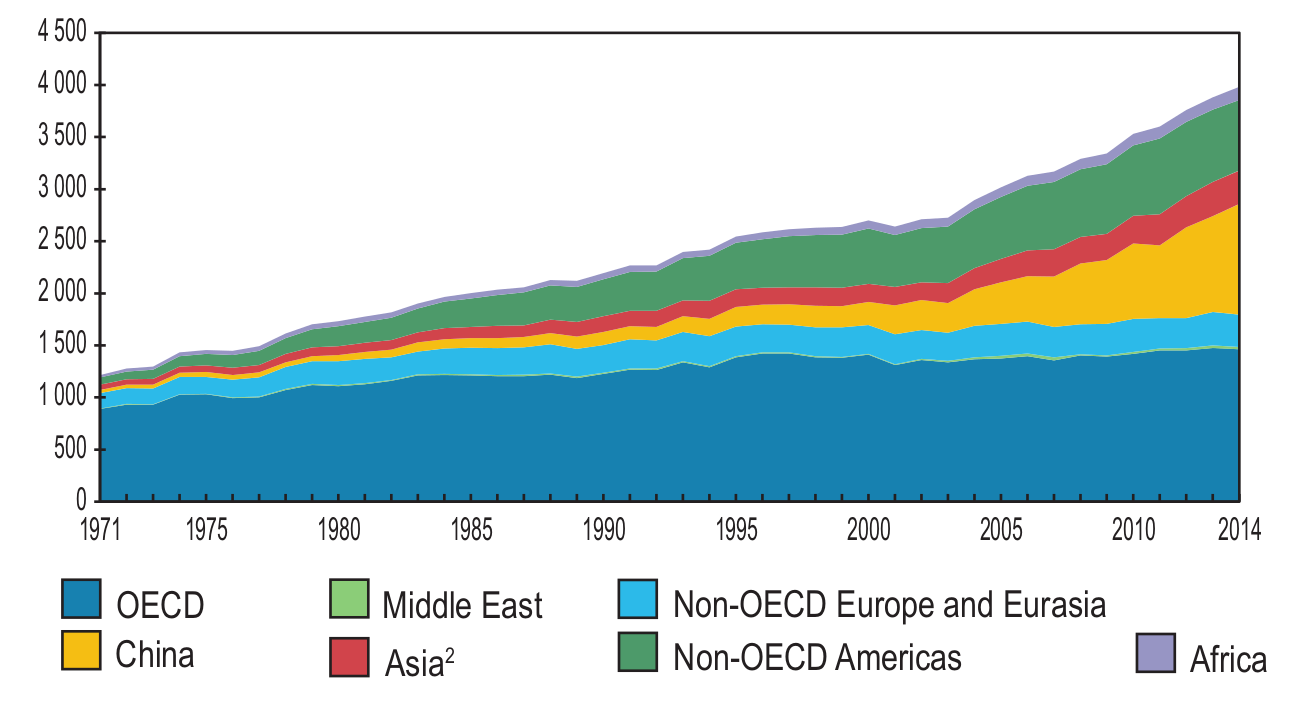
\includegraphics[width=10cm]{world_hp.png}
\caption[Hydroelectricity production by region from 1971 to 2014 in TWh]{Hydroelectricity production by region from 1971 to 2014 in TWh \cite{iea_stat}}
\label{world_hp}
\end{figure}

In Europe hydropower is the largest renewable energy resource, accounting for \unit[18]{\%} of of total electricity generation. However, the potential for hydropower generation depends on geographic and climatic conditions, and capacity is concentrated in several distinct regions, including the Nordic countries, the Alps, the Iberian Peninsula as well as Turkey \cite{hp_europe}. \newline
In Germany, hydroelectricity production is mostly concentrated in the south and west (Bayern, Baden-Württemberg, Rheinland Pfalz, North Rhine-Westphalia), as can be seen on Fig. \ref{hp_de}, based on the Open Power Data Set. In 2014, it accounted for \unit[12]{\%} of the renewable electricity production in Germany, with around \unit[20]{TWh} produced (reservoir plants, run-of-the-river plants, as well as production from natural inflow in pumped storage plants) \cite{bdew}.

\begin{figure}[H]
\centering
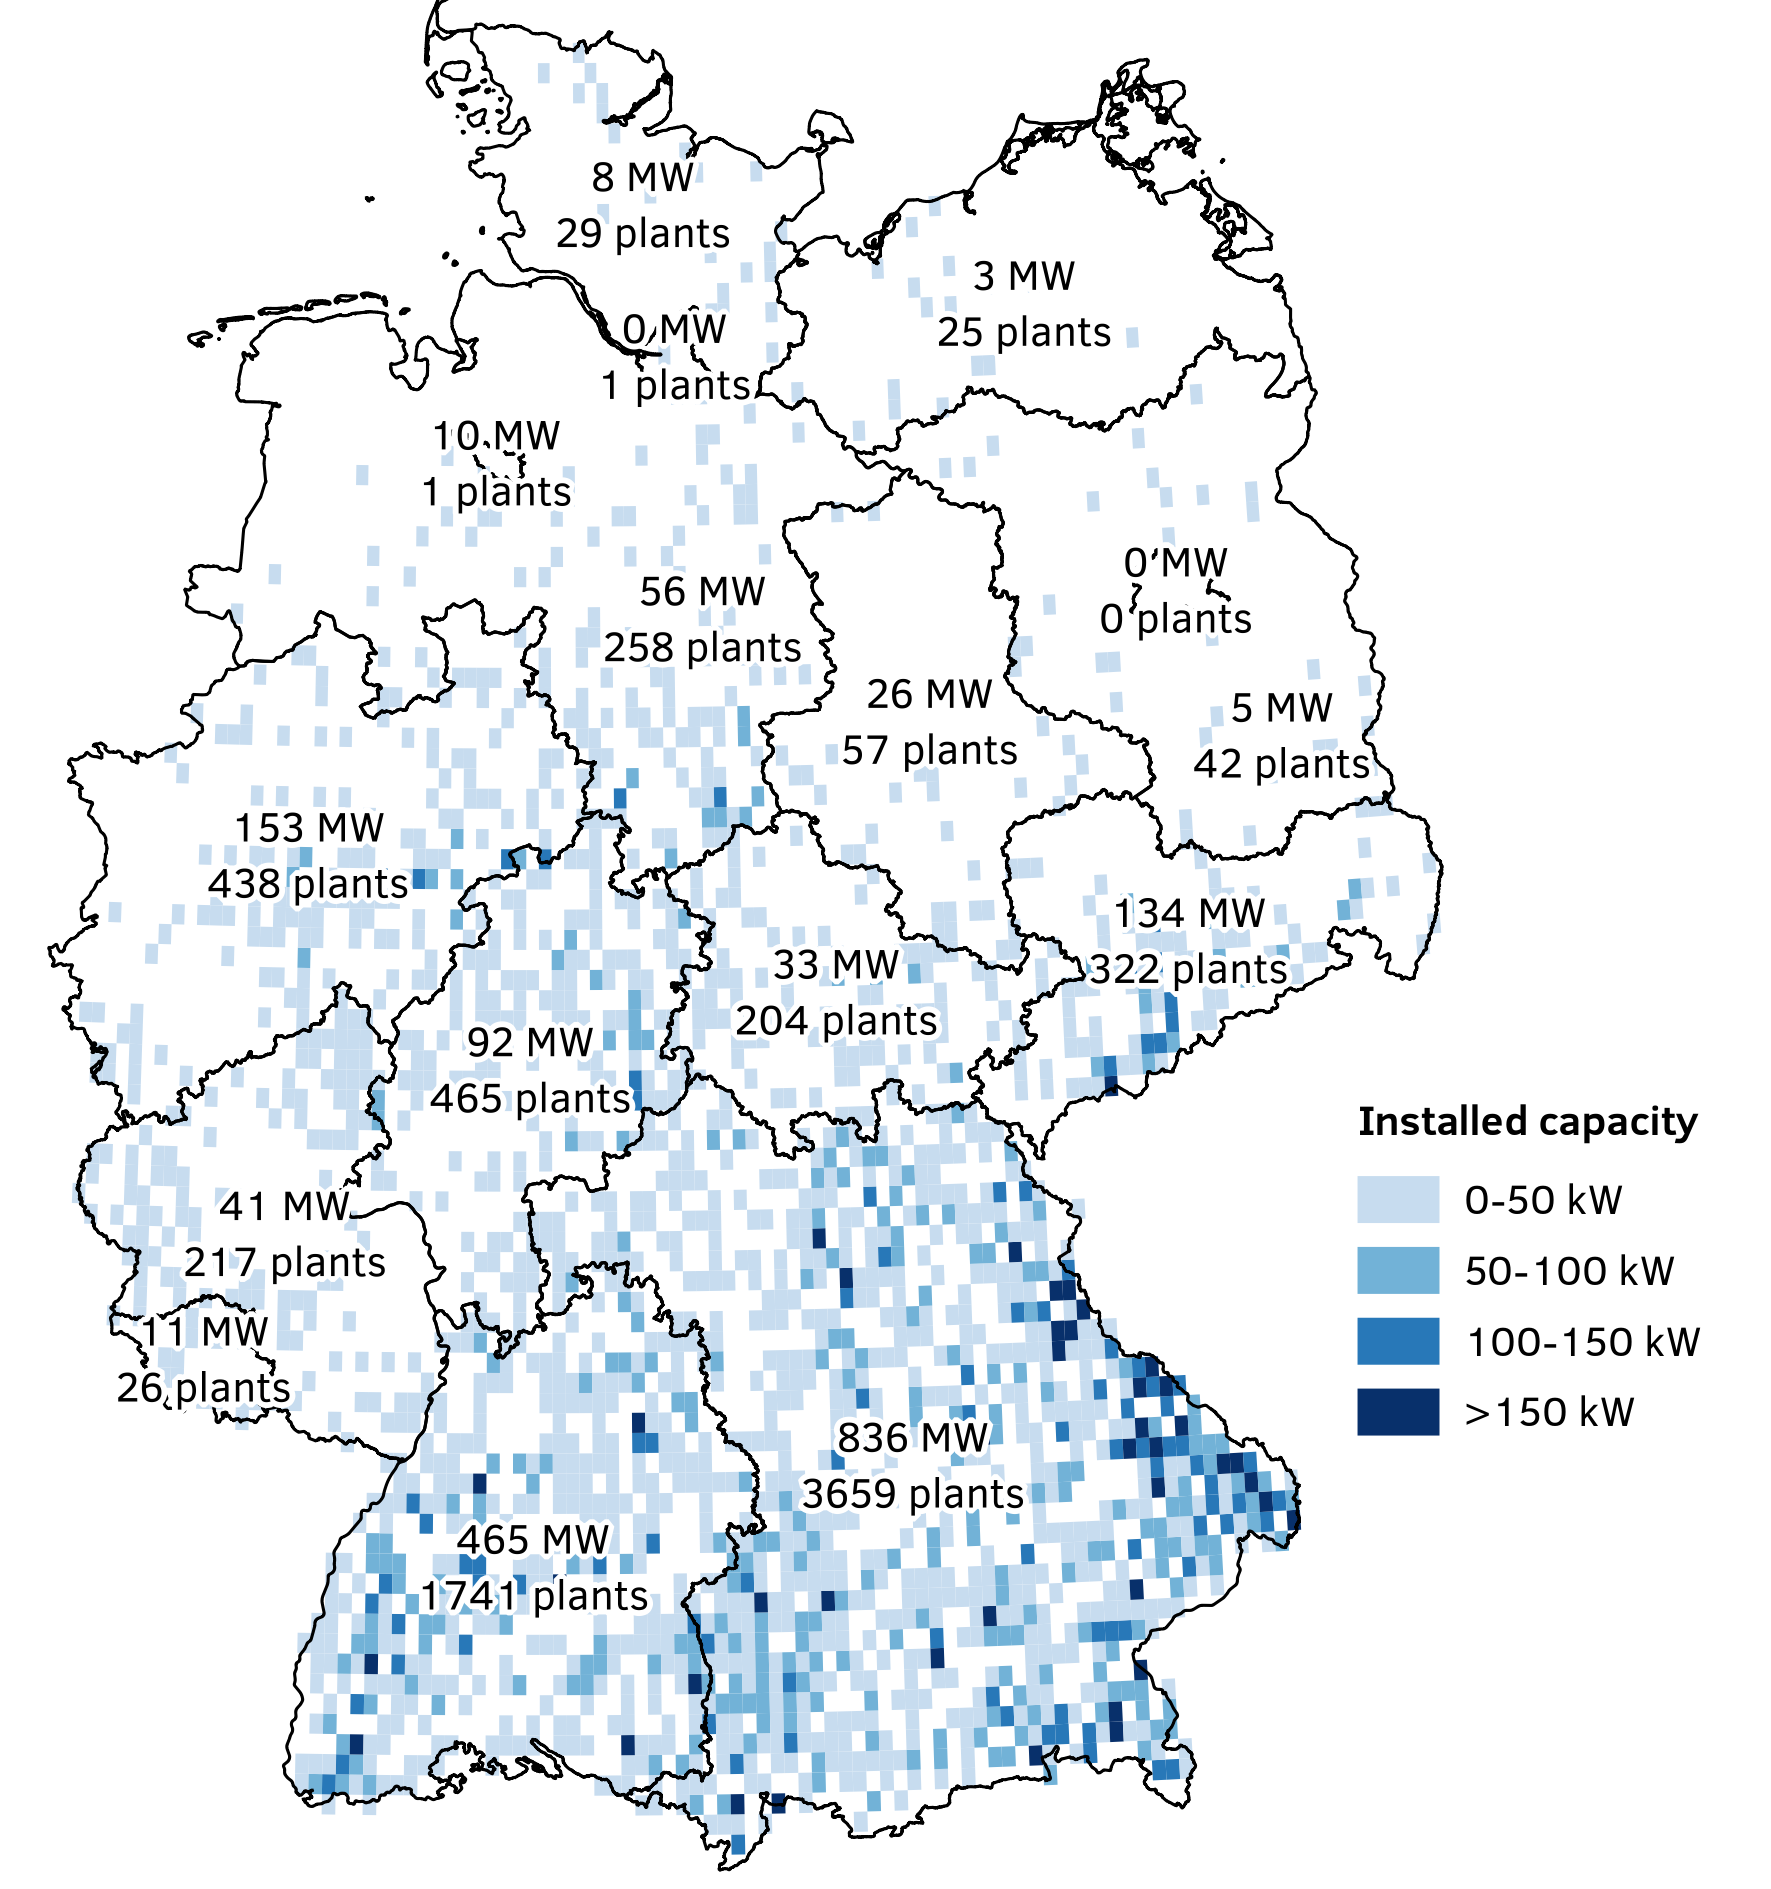
\includegraphics[width=10cm]{new_map_intro.png}
\caption[Use of hydropower in Germany]{Use of hydropower in Germany}
\label{hp_de}
\end{figure}

Reservoir hydropower plants have negative social and environmental impacts because of the changes brought by the construction of dams and reservoirs. These structures change the ecosystem, both aquatic and terrestrial, by flooding areas, destroying wildlife habitat, and changing or blocking the water flow. Reservoirs also occupy large areas and sometimes require entire communities to be relocated. Most new projects must undergo an environmental and social impact assessment to oversee, prevent or compensate the negative impacts. Run-of-the-river power plants, in contrast to reservoir plants, have a much smaller impact on the ecosystem and the society because they do not require water impoundment. The dams are often equipped with a fish ladder and fish protection facilities, in order not to impede wildlife circulation. \newline 
Hydropower presents many advantages for a transition to a more sustainable energy system : it does not require any fossil fuels in the operating phase, it has a very low life cycle GHG emissions (see Fig. \ref{ghg_em}), and it is available at a commercial scale at competitive costs \cite{hp_europe}. For this reason, it has to be taken into account in transition scenarios and energy system models. 

\begin{figure}[H]
\centering
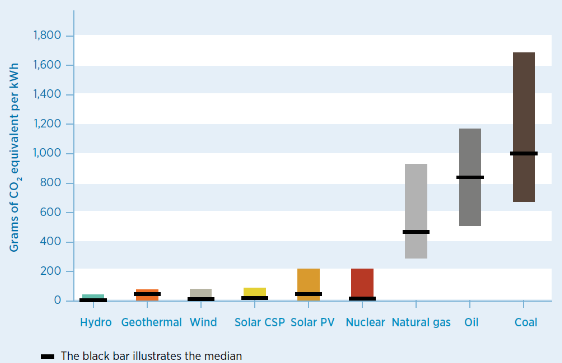
\includegraphics[width=12cm]{ghg_em.png}
\caption[Life-cycle emission intensity of electricity generation by technology]{Life-cycle emission intensity of electricity generation by technology \cite{hp_europe}}
\label{ghg_em}
\end{figure}


\section{Energy systems modeling}

In the past decades, the need for an energy transition has emerged. This need has been acknowledge in the sustainable development goals \cite{un_sdgs} set by the United Nations, in particular ``affordable and clean energy'' (goals 7) \cite{un_sdg7} and ``sustainable cities and communities'' (goal 11) \cite{un_sdg11}. However, a successful energy transition will have a positive impact on other development goals as well, through a reduction of pollution, global warming, and conflicts about the access to fossil fuels. \newline
The transition in the production of energy is made possible by replacing conventional fuels such as coal, gas or uranium by renewable energy sources, such as wind, sunlight, kinetic and potential energy of water, biomass or geothermal energy. These energy sources are harnessed on site, and the potential of a site is highly dependent on the weather, the relief, as well as the time of the year or of the day. This leads to a more decentralized and intermittent production compared to conventional power plants, which makes the energy system more complex. \newline
Because of the irregularity of the production and the strong dependance on weather, the energy supply is not controllable, and cannot always follow the demand. Furthermore, the variability in the potential of each type of renewable energy depending on the site requires an adjustment of the energy system from site to site. This prompts the need for reliable energy systems modeling to simulate and optimize the energy mix, distribution network and energy management of a given region. The simulation of energy systems requires good quality energy conversion and distribution models, consistent data about the weather, the existing plants in the region, and the energy demand, and robust optimization tools.


\section{Open source and open data}

The volume of research about renewable energy has grown over the last decades (more than 180 university and 120 non-university research institutes are conducting research about energy transition in Germany alone \cite{bmbf_energiewende}), and various actors of the energy sector are developing models and data sets for energy systems and gathering input data for these models. The complexity of the models has also increased, requiring specialists of different fields to work together (geographers, meteorologists, energy specialists, economists, sociologists, …). However the tools and databases themselves are rarely made public, which forces different actors to inject time, money and energy into developing the same models and gathering the same data. \newline
To adress this problem and promote open energy modeling in Europe, the Open Energy Modeling initiative (Openmod) was launched in September 2014 by several researchers in Germany and abroad \cite{openmod_workshop}. They strive for open science in all its forms : open source software and hardware, open data, open access to publications, open peer review, open educational resources and open methodology about all these aspects, and they state that ``more openness in energy modeling will increase transparency and credibility, reduce wasteful double-work and improve overall quality`` \cite{openmod_manifesto}. \newline
The Reiner Lemoine institute has been part of this initiative since the beginning and  carries out several projects of open energy modeling, such as oemof (open energy system modeling framework \cite{rli_oemof}), open\_eGo (open electricity grid optimization \cite{rli_openego}) or open\_FRED (open feed-in time series based on a renewable energy database \cite{rli_openfred}). 

\section{Aim and structure of the thesis}
This work is part of the open\_FRED project, which aims at creating and making available consistent standard data of all relevant data sets (power plant registers, adjusted climate data, and basic data such as river networks or administrative boundaries), and at developing compatible open source simulations models, which will produce feed-in time series of fluctuating renewable energies. \newline
Given the important part of hydropower in the european energy mix, the low life cycle GHG emissions of hydropower, and the limited environmental and social impacts of run-of-the-river hydroelectricity, a set of renewable energy models would not be complete without a model for run-of-the-river electricity production. \newline
This thesis tackles the issue of modeling and simulating electricity generation from run-of-the-river hydroelectric power plants based on open access geodatabases. It aims at developing an open-source Python model able to simulate time series of the electrical output of one or several run-of-the-river power plants based on open source data sets of power plants, weather, and river discharge. \\
Chapter \ref{chap:basics} will focus on the basic principles of hydropower, and present a state of the art of technology and research in this domain. Chapter \ref{chap:data_basis} will list the the necessary and available data sets about hydropower. Chapter \ref{chap:methodology} will present a methodology adapted to the available data in order to develop the model introduced in Ch. \ref{chap:simulation_model}. Finally, the results of the model will be presented in Ch. \ref{chap:results} and discussed in Ch. \ref{chap:discussion}.

